\section{Expected Impacts}
% one paragraph on what's current stage before my work
Currently, the techniques of immersive video streaming are still in their infancy.
% Most of the challenges mentioned in front sections haven't solved yet, especially the high bandwidth requirement.
Most of the challenges identified in this proposal have not been rigorously studied.
Existing VR/AR applications do not support real-time streaming; 
Even if they do, only 3DoF interactions are supported, which is not the {\em real} immersive experience.

% one paragraph on what it will become after my work 
In my PhD study, we will propose a series of solutions to overcome the challenges of immersive video streaming.
As system researchers, these solutions through actual experiments. 
In data representation research, we will provide a comprehensive review, 
which can help the research community gain more knowledge on the features, challenges and opportunities of various 6DoF data types.
Through user study and data analysis, we will find new discoveries on the user experience of immersive video streaming in QoE research.
With these discoveries, the content creators can better meet users' needs when they create the immersive content.
The researchers can also use the users' viewing behavior to develop more efficient streaming solutions.
In optimal streaming, we will propose innovative algorithms to overcome various issues caused by scarce resources.
The bandwidth and latency requirements of immersive video streaming will, therefore, fulfilled under diverse network conditions, and
several 6DoF applications can be realized.

\begin{figure}[tbh]
	\begin{center}
		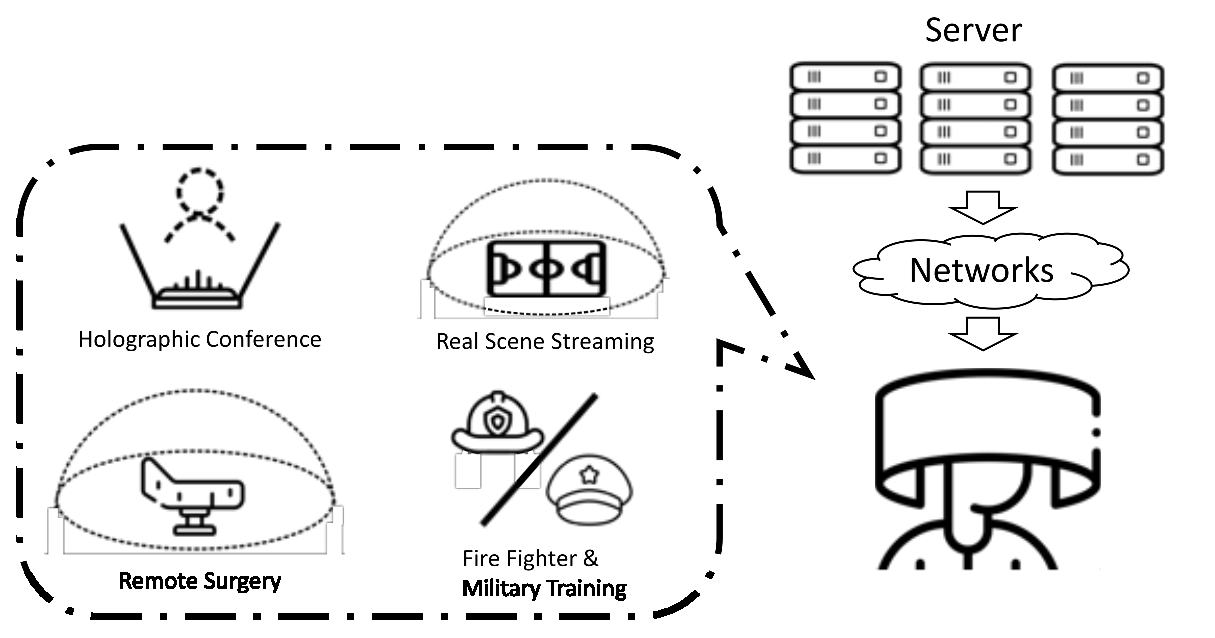
\includegraphics[width=.5\textwidth]{fig/usage_scenario}
		\caption{Usage scenario of immersive video streaming.}
		\label{fig:usage_scenario}
	\end{center}
\end{figure}

% one paragraph on how would my work change people life 
The techniques of immersive video streaming can make people's life more convenient and productive.
As shown in Fig.~\ref{fig:usage_scenario}, immersive video streaming can be used in various usage scenarios.
\begin{itemize}
    \item {\bf Holographic conferences} may become reality. 
    Users can see the projection of remote people and communicate with  one another naturally.
    The holographic conferences will provide exactly the same experience as face-by-face.
    \item {\bf Real scene streaming} may provide immersive live streaming for sports, speech, and other events. 
    For example, users can watch live sports without blind angles to enjoy the games.
    \item {\bf Remote Surgery} can also be performed. 
    Immersive video streaming can provide the situations of remote patients to 
    the doctor, who can carry out the surgery remotely. This will improve the healthcare quality in rural areas.
    \item {\bf Fire fighter and Military training} can be clone in a safer and more efficient way. 
    The training sessions can simulate real situations to help learners experience danger environments without risks.
\end{itemize}


% The usage scenario of immersive video streaming shown in Fig.~\ref{fig:usage_scenario}.
